\documentclass[10pt,a4paper]{article}
\usepackage[margin=18mm,columnsep=6mm]{geometry}
\usepackage[T1]{fontenc}\usepackage[utf8]{inputenc}\usepackage{mathptmx,microtype,graphicx,caption,amsmath}
\usepackage[numbers,sort&compress]{natbib}\usepackage[hidelinks]{hyperref}\usepackage{xurl}\setlength{\bibsep}{4pt}
\captionsetup{font=small,labelfont=bf,skip=5pt}\setlength{\parindent}{0pt}\setlength{\parskip}{5pt}
\begin{document}
\begin{center}{\LARGE\bfseries Feeding Frenzy: local rules and conditional feeding benefits in dolphin--gannet hunting\par}\vspace{6pt}Reuben Stanley | University of Western Australia\par{\small Working draft - 9 November 2026 - complete exploratory regime map}\end{center}
{\large\bfseries 1 Question and local-rule perspective\par}\vspace{7pt}
\begin{minipage}[t]{238.10999999999999pt}\vspace{0pt}
\textbf{Abstract}\par Adding another predator can expose prey while also increasing competition. We test this balance under one fixed dolphin herd--strike rule, using matched encounters with and without gannets. The original small pilots gave dolphin gains of 17.1\% and 16.1\%. A declared exploratory map varies the minimum herding interval and bird count on four previously observed schools, with species-matched controls and a stronger best-tested dolphin-only comparison. The largest mixed dolphin return occurred at H=1T with 6 birds: 91\ensuremath{\rightarrow}113 captures against same-H controls (+24.2\%); it exceeded the best-tested dolphin-only return of 91. These are discovery-bank outcomes, not a confirmed optimum. An independent eight-school check had a small coarse-grid dolphin gain whose interval included zero; halving the timestep gave no mean dolphin gain. Conditional model benefits therefore require separate numerical and biological validation.\par\smallskip
\textbf{Question}\par The South African sardine run brings several predators to the same moving resource \citep{teske2021}, \citep{odonoghue2009}. Their association does not show whether either species obtains more food than it would alone. We ask when adding gannets improves dolphin feeding while the dolphin rule remains unchanged, and separately whether gannets also benefit. The comparison begins with an already located fish school; it does not measure searching for prey or energetic profitability.\par\smallskip
\end{minipage}
\hfill
\begin{minipage}[t]{238.10999999999999pt}\vspace{0pt}
\textbf{Ecological motivation}\par Successive predator attacks can disrupt prey aggregations in models \citep{lett2014}, and underwater observations link attack history to gannet feeding success \citep{thiebault2016}. Those observations do not provide the matched dolphin-only counterfactual. Dolphins may concentrate prey for birds, while bird attacks may expose fish to dolphins. Competition and time spent herding can offset either service. Increased combined catch alone is insufficient evidence of mutual benefit.\par\smallskip
\textbf{Local rules and collective response}\par Collective-behaviour models explain how local responses can produce group-level structure \citep{couzin2002}. Here, local predator pressure and fish responses may change prey concentration, movement and accessibility, altering interception opportunities. This motivates a chain from individual rules through collective fish state and eligible contacts to captures. The chain guides diagnostics; a correlation between its stages does not establish causal mediation or intentional cooperation.\par\smallskip
\textbf{Scope and objectives}\par The main study retains one exposed-prey dolphin rule selected during development. It measures the effect of adding birds and explores conditions under which that effect changes. Matching gannet-only controls test reciprocal feeding returns. Earlier initial-depth and attack-timing pilots remain supporting investigations; the parameter map does not demonstrate depth control, a timing advantage or an unrestricted optimal hunting strategy.\par\smallskip
\end{minipage}
\clearpage
{\large\bfseries 2 Model and behavioural assumptions\par}\vspace{7pt}
\begin{minipage}{\textwidth}\centering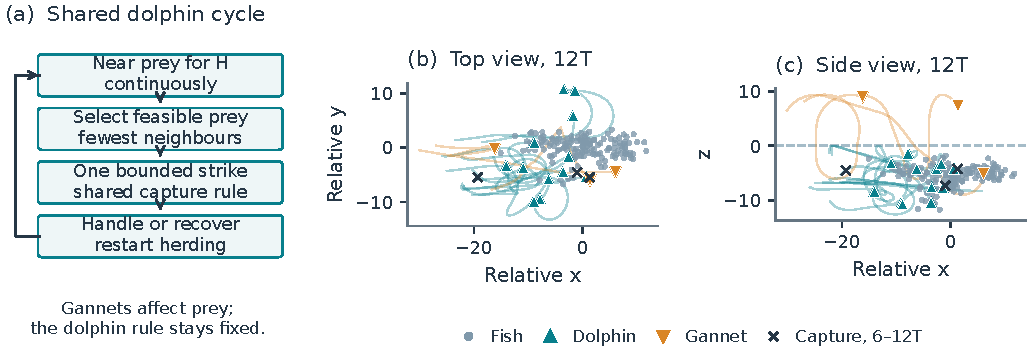
\includegraphics[width=\linewidth]{figures/fig1_model.pdf}\captionof{figure}{One shared dolphin cycle and an illustrative recorded encounter. Continuous near-prey pressure for H is followed by a feasible strike preferring fewer prey neighbours and ordinary recovery. Bird presence does not change this dolphin rule. Top and side views show original development school 39061002 at 12T; paths and captures cover 6--12T. The snapshot was fixed before the sweep and does not certify compactness, completed herding or a causal mechanism.}\end{minipage}\par\vspace{7pt}
\begin{minipage}[t]{238.10999999999999pt}\vspace{0pt}
\textbf{Fish and inherited engine}\par We use the inherited native C++ FishSim engine, with Python predator controllers, experiment harnesses and analysis added for this project. The 160 point-represented fish use separation, alignment and attraction \citep{couzin2002}, with repulsion taking priority, plus migration, habitat and predator-response terms. Horizontal space is open; water lies below z=0. Fish speed is 3 model units per T and native movement noise is zero. Nearby submerged predators change escape steering and social responses; airborne birds provide no threat cue.\par\smallskip
\textbf{Dolphin herding cycle}\par Each of 12 dolphins follows local waypoints ahead of, beside and below a tracked prey patch. A cycle requires H continuously within 4.5 units of at least one observed fish; lost proximity resets the clock. The original H=2T is extended to H=1,2 or 3T. This pressure represents a contribution to pod herding, without assigned drivers, barriers or feeding turns. It does not certify a compact baitball, complementary coverage or pressure on the same fish throughout.\par\smallskip
\end{minipage}
\hfill
\begin{minipage}[t]{238.10999999999999pt}\vspace{0pt}
\textbf{Feasible exposed-prey strikes}\par After H, a dolphin ranks feasible fish within range 6 by fewer neighbours inside radius 2, then predicted interception and turning time. Dense fish remain eligible; outward motion is not required. A strike is bounded by 6T, speed 6 and turning limit \ensuremath{\pi}/2 per T. Recovery lasts 2T after capture or 0.75T after failure. Dolphins know local fish states exactly within range 25 and receive no bird-count, dive-event or post-dive bonus. The cycle repeats with the same rule in every species-presence comparison.\par\smallskip
\textbf{Gannet perception and roster}\par Birds have idealised global prey information within detection depth 12. DBSCAN uses radius 2 and minimum neighbourhood count 4; eligible clusters are sampled by accessible fish count, then a dense accessible location is targeted. Approach, plunge, underwater pursuit, ascent and recovery remain physically constrained \citep{ropert2004}. One bird uses G0, three use G0--G2, and six add birds at those same three launch locations. Count therefore changes coverage or local multiplicity; bird body-spacing avoidance is absent.\par\smallskip
\textbf{Contact and step order}\par An eligible swept contact between point prey and an offset mouth sphere (radius 0.4, forward offset 0.3) succeeds with fixed q=0.7. The first eligible contact closes the bout whether it succeeds or fails; each captured fish is removed once. Predators propose motion from the same step-start fish state. Fish advance under submerged-predator cues, contacts resolve jointly in time order, and controller memory commits the resolved step. No density-dependent capture bonus is imposed.\par\smallskip
\end{minipage}
\clearpage
{\large\bfseries 3 Comparisons and evidence design\par}\vspace{7pt}
\begin{minipage}{\textwidth}\centering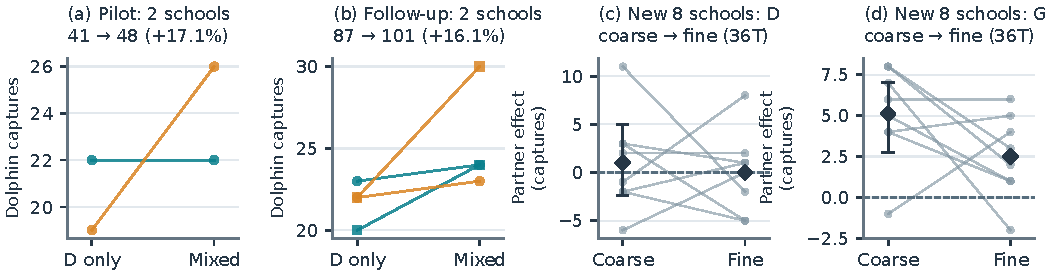
\includegraphics[width=\linewidth]{figures/fig2_cohorts.pdf}\captionof{figure}{Distinct cohorts under the same dolphin rule. Colour identifies school within each two-school panel; circles/squares identify capture-stream settings 61001/61002. Lines join dolphin-only and mixed outcomes. The development totals 41\ensuremath{\rightarrow}48 and follow-up 87\ensuremath{\rightarrow}101 involve four distinct pilot school geometries overall; the two follow-up settings do not add independent schools. Separate panels show the same eight later schools across coarse/fine 36T grids, with mean diamonds and 97.5\% marginal bootstrap intervals only for the coarse primary means. The fine check did not rerun the earlier positive cohorts.}\end{minipage}\par\vspace{7pt}
\begin{minipage}[t]{238.10999999999999pt}\vspace{0pt}
\textbf{Counterfactual and return}\par The baseline has the same dolphin number, H, target preference, physical abilities, initial readiness and private random streams, without gannets. Birds change prey dynamics and competition rather than unlocking dolphin attacks. Feeding return is Y\_s=C\_s/(N\_s T), where C\_s is uniquely removed prey and N\_s is predator abundance. All travel, herding, failed attacks and recovery count. Complete depletion fixes later food while native stepping ends; food retains the full nominal encounter denominator.\par\smallskip
\textbf{Original positive cohorts}\par The original exposed-prey development pilot gave 22\ensuremath{\rightarrow}22 and 19\ensuremath{\rightarrow}26 dolphin captures across two schools: 41\ensuremath{\rightarrow}48 overall (+17.1\%). A follow-up on two fresh schools, each under two stream settings, gave 87\ensuremath{\rightarrow}101 (+16.1\%), with all four differences positive. These are two independent schools per cohort, not one independent unit per repetition. The controller was chosen during development; subsequent same-rule partner tests do not establish policy optimality.\par\smallskip
\textbf{Independent replication and grids}\par Eight further schools were declared before feeding outcomes and passed fixed predator-free stability and route screens. Each had matched D-only, G-only and mixed encounters with 160 fish, 12 dolphins and/or 3 gannets. Coarse runs used dt=0.00125T and 72T, with 36T prespecified as primary. Fine runs reused the same physical starts, actor states and private-stream initialisations at dt=0.000625T for 36T. They are paired numerical treatments of eight schools, not 16 independent schools. Halving dt doubles the 36T updates from 28,800 to 57,600 without changing hunting duration.\par\smallskip
\end{minipage}
\hfill
\begin{minipage}[t]{238.10999999999999pt}\vspace{0pt}
\textbf{Declared exploratory map}\par The corrected-v2 map comprises 60 condition-school executions: H={1,2,3}T crossed with G={0,1,3,6} for each of four previously observed schools, plus G-only controls at each positive bird count. All use 36T, the original coarse timestep, one capture-stream setting and fixed q=.7. Eight H2/G0-or-G3 executions must reproduce archived outcomes exactly before the other 52 run. These replays add no independent evidence. A stopped recorder-diagnostic attempt remains immutable provenance and is excluded. Schools share sampler parameters but differ in evolved positions and headings after 20T preparation; school seeds also initialise readiness and private streams.\par\smallskip
\textbf{Pairing, uncertainty and selection}\par The primary dolphin effect is mixed minus same-H D-only return. The reciprocal effect uses per-bird return against same-count G-only controls, shared across H. A fixed 10,000-draw bootstrap resamples whole four-school vectors across the entire map. Its 95\% intervals are exploratory and pointwise, without multiplicity correction. A stronger secondary comparison chooses the highest-mean D-only H across this discovery bank, with smaller-H ties, and reselects it within each draw; it is not a per-school oracle or global optimum.\par\smallskip
\end{minipage}
\clearpage
{\large\bfseries 4 Complete parameter response\par}\vspace{7pt}
\begin{minipage}{\textwidth}\centering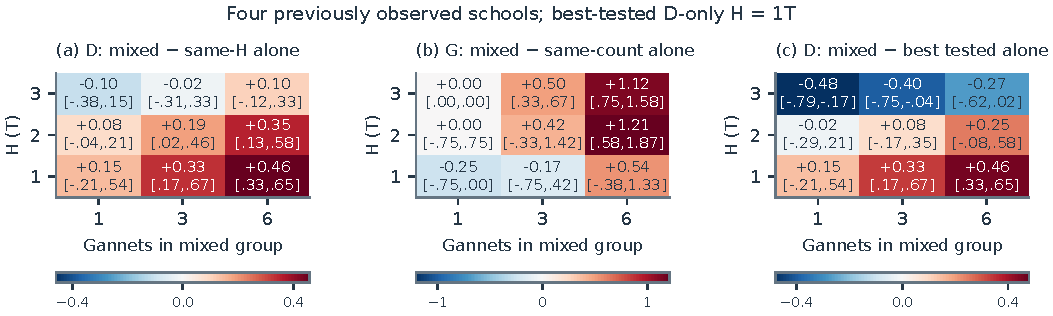
\includegraphics[width=\linewidth]{figures/fig3_regime_map.pdf}\captionof{figure}{Complete declared H\ensuremath{\times}G response map on four previously observed schools. Mean paired changes and pointwise 95\% whole-school bootstrap intervals are shown per predator over the full 36T encounter. Comparators are same-H D-only, same-count G-only and the best-tested D-only H chosen across this discovery bank and reselected within each draw. All nine mixed settings and signs are retained; all 36 school contrasts and absolute returns are in the notebook. Panels use separate symmetric colour ranges. Selected large cells are exploratory discoveries, not confirmed optima.}\end{minipage}\par\vspace{7pt}
\begin{minipage}[t]{238.10999999999999pt}\vspace{0pt}
\textbf{Whole-map outcome}\par All 60 declared executions, eight exact anchor replays and physical/raw-event audits passed. Across the nine mixed settings, mean same-H dolphin effects were positive in 7, zero in 0 and negative in 2. Mixed dolphin food ranged from 1.42 to 2.35 captures per dolphin over 36T. Figure 3 retains the entire map, not only its largest response.\par\smallskip
\textbf{Dolphin response at fixed behaviour}\par The largest observed mixed dolphin return was at H=1T and 6 gannets, chosen by mixed mean food with fewer-bird and smaller-H tie rules. Across four schools, D-only and mixed totals were 91 and 113 (+24.2\%); school differences were +4, +9, +4, +5 fish. The equal-school mean same-H change was +0.46 captures per dolphin per 36T, with pointwise 95\% interval [+0.33, +0.65]. This in-sample selection is exploratory.\par\smallskip
\textbf{Gannet and joint returns}\par Mean count-matched per-bird effects were positive in 5 of nine settings, zero in 2 and negative in 2. At the selected dolphin-return setting, the mean gannet change was +0.54 captures per bird per 36T, interval [-0.38, +1.33]; raw gannet school differences were -5, +6, +2, +10. Both species gained in 3/4 schools there. At H=2T with 6 birds, dolphins changed 86\ensuremath{\rightarrow}103 and gannets 24\ensuremath{\rightarrow}53, with both gaining in all four schools. Its dolphin interval against the stronger best-H benchmark crossed zero.\par\smallskip
\end{minipage}
\hfill
\begin{minipage}[t]{238.10999999999999pt}\vspace{0pt}
\textbf{Stronger dolphin-only benchmark}\par The highest across-school dolphin-only mean occurred at H=1T, with 91 captures across four schools. The selected mixed setting produced 113 (+24.2\%), a mean change of +0.46 captures per dolphin per 36T against this stronger benchmark, interval [+0.33, +0.65]. The bootstrap reselects H within each school-vector draw. This is the best tested herding minimum for the retained rule, not an optimum across all dolphin behaviour.\par\smallskip
\textbf{What the map can establish}\par These four starting geometries were already observed in the pilots. The map explores the chosen rule after positive outcomes; it is not fresh independent confirmation. Reused controls and exact replay executions do not multiply replication. Every declared cell, including zero and negative responses, is reported. Pointwise intervals from n=4 do not correct selection of the largest observed response. Any conditional benefit is specific to this discovery bank, fixed q, bird roster and coarse timestep.\par\smallskip
\end{minipage}
\clearpage
{\large\bfseries 5 Collective state, opportunities and robustness\par}\vspace{7pt}
\begin{minipage}{\textwidth}\centering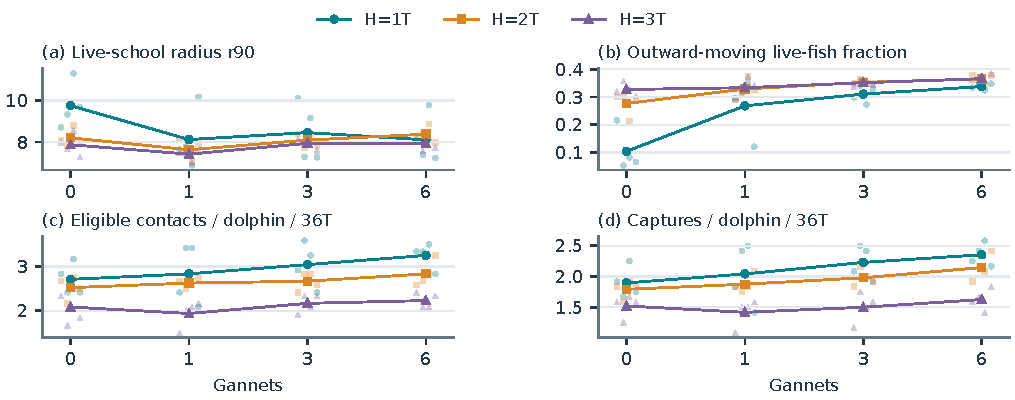
\includegraphics[width=\linewidth]{figures/fig4_diagnostics.pdf}\captionof{figure}{Descriptive response across every dolphin-bearing H\ensuremath{\times}G setting, including G=0. Faint points show all four schools and lines show equal-school means. Live-fish r90 and outward fraction are time-averaged over observed nonempty saved frames without selected post-dive windows. Eligible contacts and captures use the full 36T denominator. Prey removal and survivor selection can change fish-state summaries; these associations do not establish causal mediation, completed herding or biological cooperation.}\end{minipage}\par\vspace{7pt}
\begin{minipage}[t]{238.10999999999999pt}\vspace{0pt}
\textbf{Collective fish state}\par Across all 12 dolphin-bearing settings, equal-school time-mean live-fish r90 ranged from 7.42 to 9.76 model units, while mean outward-moving fractions ranged from 0.104 to 0.366. Figure 4 shows every school and H, with no selected post-dive window. These state summaries are conditional on surviving fish and observed nonempty frames; they do not certify whole-school containment or isolate the effect of bird disturbance.\par\smallskip
\textbf{Contact opportunities and food}\par At H=1T and 6 birds, pooled dolphin eligible contacts changed from 130 to 156, launches from 251 to 267, and food from 91 to 113 across the same four schools. These descriptive changes occurred under the same conditional success rule. The realised capture-to-contact ratio describes eligible contacts and random draws; it is not a fitted field attack-success parameter. Saved-state and event diagnostics can reveal where responses change, but they do not separate disturbance, competition and selection of surviving prey into causal effects.\par\smallskip
\textbf{Numerical sensitivity remains}\par In the independent eight-school coarse 36T primary test, dolphins captured 168 alone and 176 mixed; gannets captured 35 and 76. Mean effects were +1.00 dolphin and +5.125 gannet captures per school; 97.5\% marginal intervals were -2.375 to +5 and +2.75 to +7. Halving dt gave dolphins 179\ensuremath{\rightarrow}179 and gannets 49\ensuremath{\rightarrow}69. The zero dolphin mean includes four positive, three negative and one zero school effect; it does not mean every school lost its benefit. Dolphin effect signs agreed in 3/8 schools and gannet signs in 6/8. Three schools had joint gains on each grid, but only two overlapped. This check did not refine the original positive cohorts or the new sweep.\par\smallskip
\end{minipage}
\hfill
\begin{minipage}[t]{238.10999999999999pt}\vspace{0pt}
\textbf{Longer encounters and validation}\par At coarse 72T, the same eight-school trajectories gave dolphin totals 352\ensuremath{\rightarrow}380 and gannet totals 85\ensuremath{\rightarrow}149, with joint gains in 5/8 schools. None fully depleted the prey. These are secondary continuations, not additional replicates, and 72T was not repeated on the fine grid. A separate held-out plan would freeze a selected mixed setting and D-only benchmark before fresh outcomes. No held-out result is included here, and the exploratory map does not establish convergence.\par\smallskip
\textbf{Earlier depth and timing checks}\par Earlier G-only depth translations on two schools showed no monotonic fall in food: native fish movement changed accessibility during encounters. They test transient initial states, not maintained-depth exclusion. An isolated timing implementation reproduced its disabled baseline; a post-hoc 36T engineering check partially deferred one dive, then lost locality, with captures unchanged. Full depth, timing and source receipts remain in the notebook. Neither side investigation establishes the mechanism behind a sweep response.\par\smallskip
\end{minipage}
\clearpage
{\large\bfseries 6 Discussion and conclusion\par}\vspace{7pt}
\begin{minipage}[t]{238.10999999999999pt}\vspace{0pt}
\textbf{Conditional feeding benefits}\par The map shows 7/9 positive mean same-H dolphin responses within four known schools. Its largest mixed return exceeded the best-tested D-only benchmark (113 versus 91 captures). That comparison includes selection and small-sample uncertainty; the full response map and school points are needed to assess it. The original positive pilots remain valid observations of this implemented rule, while the independent replication shows that their gains need not persist across schools or numerical grids. A dolphin gain and a reciprocal gannet gain are separate outcomes; neither follows automatically from increased combined food.\par\smallskip
\textbf{Behavioural and numerical limits}\par Near-prey duration is a simplified herding proxy, local prey information is exact and bird perception is idealised. Point-represented prey and absent predator body spacing affect opportunities. The eligible-contact probability 0.7 is uncalibrated for both species; the field gannet success figures 13\% and 36\% refer to observed attack techniques \citep{thiebault2016}, not first/second attempts or conditional mouth contacts. Large trajectory and sign changes after halving dt prevent a numerical-convergence claim.\par\smallskip
\textbf{Discovery and future validation}\par The sweep is benefit-motivated exploration following development, not a claim that no outcome-informed selection occurred. The eight-school replication alone retained its declared model and sample without outcome-dependent changes. Any future validation must freeze the selected H, bird count and D-only benchmark before examining new schools, retain same-H partner effects as primary, and distinguish numerical sensitivity from independent biological replication. One stochastic setting per discovery school cannot partition starting-state effects from random variation.\par\smallskip
\end{minipage}
\hfill
\begin{minipage}[t]{238.10999999999999pt}\vspace{0pt}
\textbf{Biological interpretation}\par Time and length lack a validated joint physical scale. Captures exclude energetic costs, fatigue, hunger, satiety and learning; finite prey are not replenished. Feeding return is therefore neither energetic profitability nor fitness. Literature on non-coordinating predators \citep{mohapatra2025} and seabird associations with subsurface predators \citep{licht2026} also cautions against interpreting association or a model gain as deliberate communication or reciprocal cooperation.\par\smallskip
\textbf{Software and reproducibility}\par Fish dynamics inherit the native C++ engine at https://github.com/yangyushi/FishSim; this project supplies Python predator control, experimental design and analysis. The updated notebook preserves 72 earlier feeding executions and adds 60 sweep executions, including 8 exact historical replays. Its 21 default code cells rebuild four figures and export 19 tables without native simulation. An additive, separately tested runner covers the eight-school H2 coarse/fine model, not the sweep; platform and validation limits are explicit. Original manifests, source closures and stopped-attempt provenance remain intact. Code: https://github.com/reuben-trade/FishSim-Dolphin-Gannet-Pilot.\par\smallskip
\textbf{Conclusion}\par The original shared-rule pilots showed dolphin gains of 17.1\% and 16.1\%. The declared map now reports all nine mixed regimes and their controls: 7 have positive mean same-H dolphin effects, with the largest mixed return at H=1T and 6 birds (91\ensuremath{\rightarrow}113 against same-H D-only). These are conditional discovery-bank results; numerical sensitivity and held-out validation remain unresolved. A local-rule model can identify conditions worth testing, but these finite, uncalibrated encounters do not establish general mutual facilitation, energetic profitability or biological cooperation.\par\smallskip
\end{minipage}
\twocolumn\bibliographystyle{unsrtnat}\bibliography{references}
\end{document}
